
% ==============================================================================
% CAPÍTULO 4
% RESULTADOS Y DISCUSIÓN
% WALO: Localización de fuentes de ondas acústicas
% ==============================================================================

\section{Resultados y discusión}
\label{sec:resultados_discusion}

En este capítulo se evalúa el comportamiento de WALO a partir de
tres experimentos complementarios. El primero estudia la respuesta
del sistema frente a variaciones de distancia; el segundo evalúa
la estimación de dirección de llegada mediante diferencias de fase
y de tiempo; y el tercero aborda la reconstrucción cinemática de
una fuente móvil a partir del efecto Doppler.

La presentación de los resultados sigue la secuencia física de
obtención de información: primero se caracteriza la respuesta
acústica, después se examina la capacidad de estimación angular
y, finalmente, se considera la reconstrucción del movimiento.
En cada experimento se presentan las observaciones y su
interpretación, junto con las limitaciones relevantes.

% ==============================================================================
% 4.1 EXPERIMENTO 01
% ==============================================================================

\subsection{Caracterización de la respuesta espacial: Experimento 01}
\label{subsec:exp01}

El primer experimento estudia la dependencia de la señal acústica
registrada con la distancia entre la fuente y los micrófonos.
El propósito es caracterizar la respuesta radial del sistema y
examinar si las magnitudes extraídas de las señales permiten
obtener información sobre la separación entre emisor y receptor.

\subsubsection{Calibración de amplitud RMS}

Para caracterizar la respuesta en amplitud se considera el valor
RMS de la señal registrada en cada canal. En condiciones de
propagación aproximadamente esférica y para una fuente puntual
en campo libre, la amplitud de presión acústica presenta una
dependencia inversa con la distancia:

\begin{equation}
    A_{\mathrm{RMS}}(r) \propto \frac{1}{r}.
    \label{eq:exp01_amplitude_model}
\end{equation}

En consecuencia, puede examinarse la relación entre la amplitud
medida y el inverso de la distancia mediante un ajuste lineal.
La Figura~\ref{fig:exp01_amplitude} presenta la calibración
obtenida para los dos canales de recepción.

\begin{figure}[htbp]
    \centering
    \includegraphics[width=0.95\textwidth]
    {figures/exp01_fig1_amplitude_calibration.pdf}
    \caption{
        Calibración de la amplitud RMS en función del inverso
        de la distancia para los dos canales de recepción.
    }
    \label{fig:exp01_amplitude}
\end{figure}

Los ajustes lineales permiten describir la respuesta de amplitud
de cada canal dentro del intervalo de distancias evaluado.
Los coeficientes de calibración reportados para esta caracterización
son:

\begin{align}
    k_{A,1} &= 20.6934\ \mathrm{mV\,m}, &
    R_1^2 &= 0.99443, \\
    k_{A,2} &= 18.8589\ \mathrm{mV\,m}, &
    R_2^2 &= 0.99266.
\end{align}

La diferencia entre los coeficientes indica que ambos canales
no presentan exactamente la misma respuesta en amplitud.
Esta diferencia puede estar relacionada con la sensibilidad
de los micrófonos, las etapas de acondicionamiento y las
características particulares de cada canal de adquisición.

Los coeficientes de determinación muestran una correspondencia
lineal elevada para los datos utilizados en la calibración.
Sin embargo, este ajuste describe el comportamiento observado
en las condiciones experimentales consideradas y no implica
por sí mismo que la relación se conserve fuera del intervalo
caracterizado.

\subsubsection{Predicción de distancia}

Una vez caracterizada la dependencia de la amplitud con la
distancia, puede plantearse el problema inverso: estimar la
separación entre la fuente y el receptor a partir de la amplitud
RMS registrada.

La Figura~\ref{fig:exp01_distance_mock} presenta una primera
visualización de este procedimiento. Esta figura corresponde
a una versión sintética de la predicción y se incorpora
exclusivamente para evaluar la organización gráfica y
argumental del apartado.

\begin{figure}[htbp]
    \centering
    \includegraphics[width=0.95\textwidth]
    {figures/exp01_fig3_distance_prediction_MOCK.pdf}
    \caption{
        Predicción de distancia a partir de la amplitud RMS.
        Visualización sintética utilizada para ilustrar el
        procedimiento de inversión de la calibración.
    }
    \label{fig:exp01_distance_mock}
\end{figure}

La inversión de la relación de calibración permite obtener una
estimación de distancia a partir de una amplitud medida.
No obstante, la incertidumbre de esta estimación depende tanto
de la dispersión de las mediciones como de la estabilidad de
la respuesta de cada canal.

La figura presentada no constituye una evaluación experimental
de la precisión de la estimación. Para establecer dicha precisión
será necesario reemplazar esta visualización por la reconstrucción
obtenida a partir de las mediciones reales.

\subsubsection{Caracterización mediante tiempo de llegada}

Además de la amplitud, el tiempo de llegada de la señal constituye
una magnitud de interés para estimar distancias. En un modelo
de propagación directa, el tiempo de vuelo está relacionado
con la separación entre fuente y receptor mediante la velocidad
del sonido.

La Figura~\ref{fig:exp01_toa} presenta la caracterización
realizada a partir del observable temporal.

\begin{figure}[htbp]
    \centering
    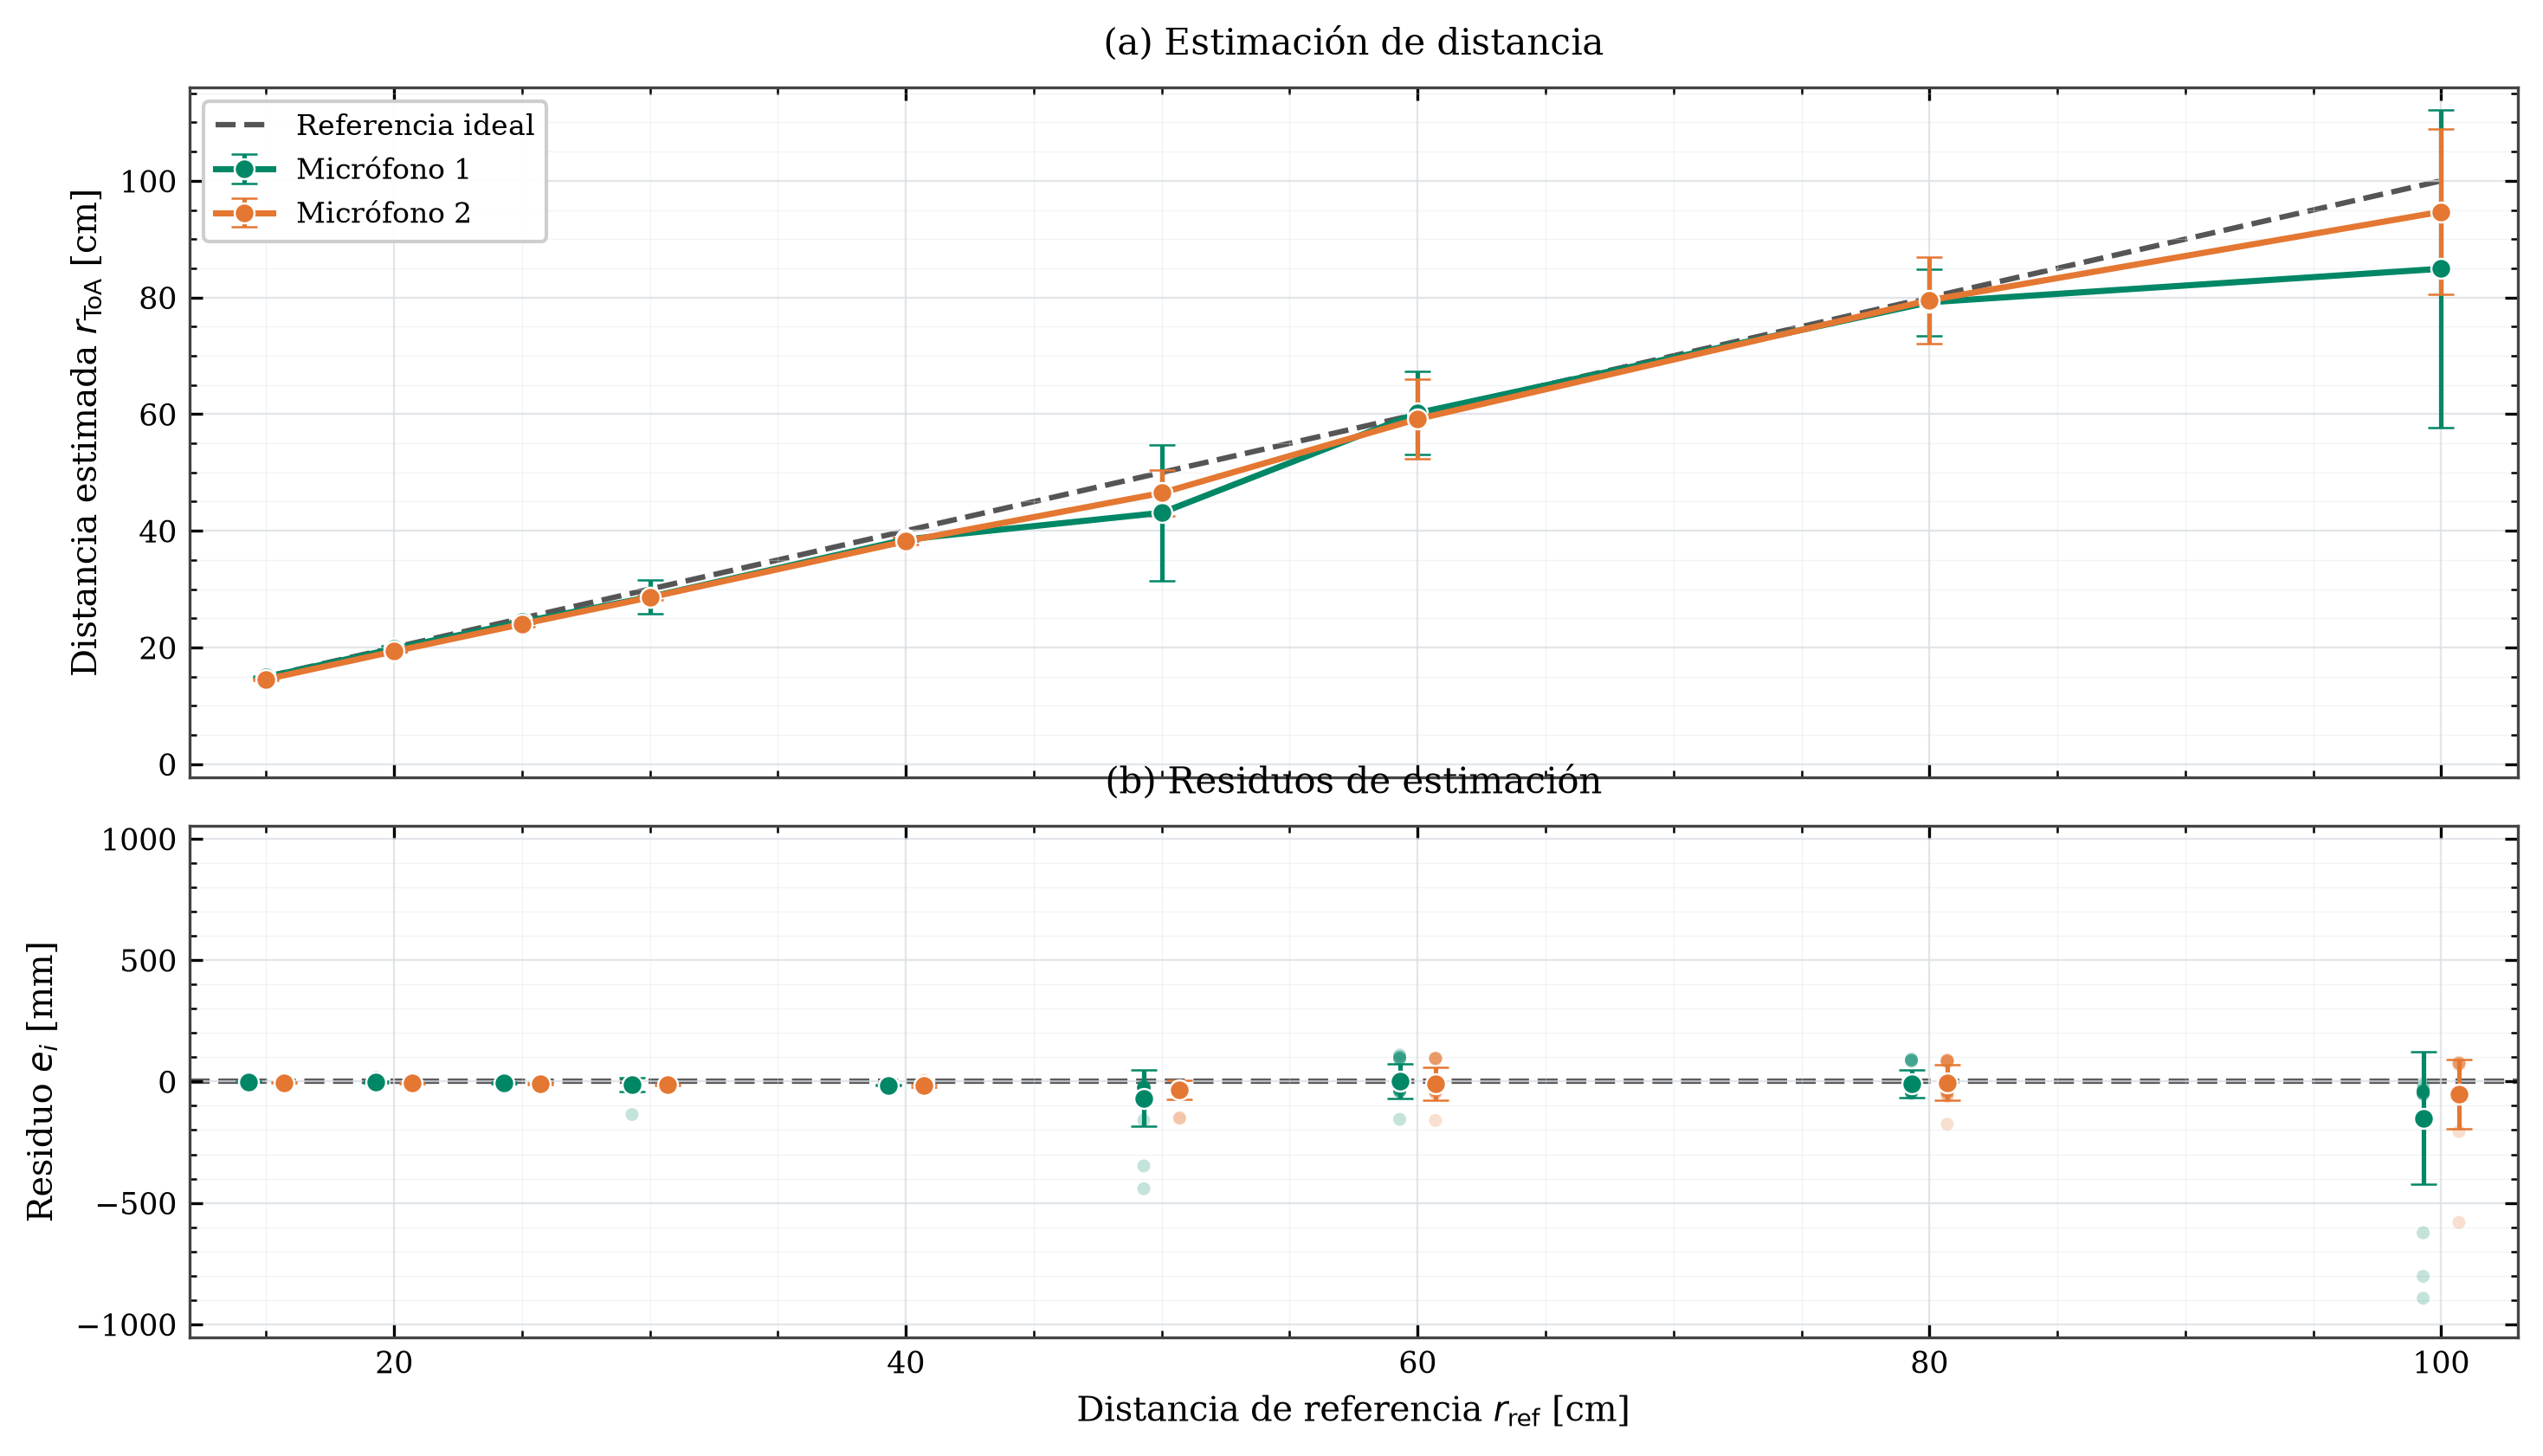
\includegraphics[width=0.95\textwidth]
    {figures/exp01_fig4_toa_range.png}
    \caption{
        Caracterización del alcance mediante el tiempo de llegada
        de la señal acústica.
    }
    \label{fig:exp01_toa}
\end{figure}

La utilidad de este observable depende de la identificación
consistente del instante de llegada y de la referencia temporal
empleada durante la adquisición. En particular, los retardos
introducidos por el sistema de adquisición y el criterio utilizado
para identificar el inicio de la señal pueden afectar la
estimación de distancia.

Por esta razón, el tiempo de llegada debe interpretarse teniendo
en cuenta tanto la propagación acústica como la respuesta temporal
del sistema de medición.

En conjunto, este experimento permite caracterizar dos aspectos
de la respuesta radial: la variación de amplitud con la distancia
y la información temporal asociada a la propagación. Ambos
observables proporcionan información complementaria, aunque
su utilización cuantitativa requiere considerar las condiciones
de calibración y las limitaciones instrumentales.

% ==============================================================================
% 4.2 EXPERIMENTO 02
% ==============================================================================

\subsection{Caracterización angular y comparación de métodos:
Experimento 02}
\label{subsec:exp02}

El segundo experimento evalúa la capacidad de WALO para estimar
la dirección de llegada de una fuente acústica. Para ello se
comparan dos métodos de estimación angular: la diferencia de
fase entre canales (PDoA) y la diferencia temporal de llegada
(TDoA).

El conjunto de mediciones comprende nueve posiciones angulares,
distribuidas entre $-60^\circ$ y $60^\circ$, con intervalos
de $15^\circ$. Para cada posición se realizaron diez mediciones,
obteniéndose un total de 90 registros válidos.

\subsubsection{Benchmark de estimación angular}

La primera comparación considera los ángulos de referencia
y las estimaciones obtenidas mediante ambos métodos.
La Figura~\ref{fig:exp02_benchmark} presenta el comportamiento
de los estimadores a lo largo del intervalo angular evaluado.

\begin{figure}[htbp]
    \centering
    \includegraphics[width=0.95\textwidth]
    {figures/exp02_fig1_angle_benchmark.pdf}
    \caption{
        Comparación entre los ángulos de referencia y las
        estimaciones obtenidas mediante PDoA y TDoA.
    }
    \label{fig:exp02_benchmark}
\end{figure}

La comparación permite examinar la correspondencia entre
la dirección de referencia y la dirección estimada.
La proximidad respecto a la relación ideal entre ambas
magnitudes constituye un indicador visual del comportamiento
de cada método.

Para complementar esta comparación se utilizan métricas
globales calculadas a partir de los residuos angulares.

\subsubsection{Reconstrucción geométrica angular}

La estimación de dirección puede representarse geométricamente
mediante la reconstrucción de las semirrectas asociadas a
los ángulos obtenidos por los dos métodos.

La Figura~\ref{fig:exp02_rays} presenta la reconstrucción
geométrica bidimensional. Esta representación permite visualizar
la orientación estimada respecto a la geometría de referencia
del experimento.

\begin{figure}[htbp]
    \centering
    \includegraphics[width=0.95\textwidth]
    {figures/exp02_fig2_ray_reconstruction.pdf}
    \caption{
        Reconstrucción geométrica bidimensional de las direcciones
        estimadas mediante PDoA y TDoA.
    }
    \label{fig:exp02_rays}
\end{figure}

La reconstrucción representa direcciones de llegada y no debe
interpretarse, por sí sola, como una localización cartesiana
completa de la fuente. Para obtener una posición espacial
es necesario incorporar información adicional, como una
estimación de distancia o una segunda restricción geométrica
independiente.

\subsubsection{Residuos y métricas de estimación}

Para cuantificar las diferencias entre las estimaciones
y los ángulos de referencia se define el residuo angular como

\begin{equation}
    e_i =
    \operatorname{atan2}
    \left[
        \sin(\hat{\theta}_i-\theta_{\mathrm{ref},i}),
        \cos(\hat{\theta}_i-\theta_{\mathrm{ref},i})
    \right],
    \label{eq:exp02_angular_residual}
\end{equation}

donde $\hat{\theta}_i$ corresponde al ángulo estimado y
$\theta_{\mathrm{ref},i}$ al ángulo de referencia.

Esta definición permite expresar la diferencia angular
considerando la periodicidad de la variable. A partir de
los residuos se calculan el sesgo medio, el error absoluto
medio (MAE) y la raíz del error cuadrático medio (RMSE).

Los resultados globales disponibles se presentan en la
Tabla~\ref{tab:exp02_metrics}.

\begin{table}[htbp]
    \centering
    \caption{
        Métricas globales de estimación angular para los métodos
        PDoA y TDoA.
    }
    \label{tab:exp02_metrics}
    \begin{tabular}{lcc}
        \hline
        \textbf{Métrica} &
        \textbf{PDoA} &
        \textbf{TDoA} \\
        \hline
        Sesgo medio [$^\circ$] & 0.320 & 2.731 \\
        MAE [$^\circ$]         & 4.020 & 7.856 \\
        RMSE [$^\circ$]        & 6.223 & 12.098 \\
        Desviación estándar [$^\circ$] & 6.249 & 11.852 \\
        \hline
    \end{tabular}
\end{table}

La Figura~\ref{fig:exp02_residuals} permite examinar la
distribución de los residuos angulares y comparar la dispersión
de ambos métodos.

\begin{figure}[htbp]
    \centering
    \includegraphics[width=0.95\textwidth]
    {figures/exp02_fig3_angular_residuals.pdf}
    \caption{
        Distribución de los residuos angulares obtenidos
        mediante PDoA y TDoA.
    }
    \label{fig:exp02_residuals}
\end{figure}

Los resultados muestran un menor error absoluto medio y
un menor RMSE para PDoA en el conjunto de mediciones evaluado.
El sesgo medio también presenta un valor más próximo a cero.
Por tanto, bajo las condiciones experimentales consideradas,
PDoA presenta un mejor desempeño global que TDoA.

La diferencia entre los métodos no debe atribuirse exclusivamente
a sus modelos geométricos. También pueden intervenir la
resolución temporal de adquisición, la estimación de fase,
la relación señal-ruido y la sensibilidad de cada procedimiento
a las condiciones de propagación.

La desviación estándar reportada complementa las métricas
de error al describir la dispersión de las estimaciones.
Su interpretación debe distinguirse del sesgo: un estimador
puede presentar un sesgo reducido y, simultáneamente,
una dispersión apreciable.

En consecuencia, la evaluación angular requiere considerar
conjuntamente la exactitud y la dispersión de las estimaciones.

% ==============================================================================
% 4.3 DISCUSIÓN TRANSVERSAL
% ==============================================================================

\subsection{Discusión transversal}
\label{subsec:discusion_transversal}

Los experimentos anteriores examinan dos aspectos distintos
del problema de localización acústica. El primero estudia
la dependencia de la respuesta registrada con la distancia,
mientras que el segundo evalúa la estimación de dirección
de llegada mediante dos observables independientes.

La caracterización radial muestra que la amplitud RMS contiene
información relacionada con la separación entre la fuente
y el receptor. Sin embargo, la conversión de amplitud en
distancia requiere una calibración específica y depende
de la estabilidad de la respuesta instrumental. Por su parte,
el tiempo de llegada proporciona una vía alternativa basada
en el tiempo de propagación, cuya interpretación exige
controlar las referencias temporales y los retardos del sistema.

En el caso angular, la comparación entre PDoA y TDoA muestra
diferencias en el desempeño de los estimadores. Para el conjunto
de mediciones considerado, PDoA presenta menores valores
de MAE y RMSE. Este resultado indica que, en las condiciones
evaluadas, la estimación basada en diferencia de fase ofrece
una correspondencia más próxima con los ángulos de referencia.

Ambos experimentos evidencian que la reconstrucción espacial
depende de la calidad de los observables acústicos y de
la correspondencia entre los modelos de inversión y las
condiciones reales de medición. La amplitud, el tiempo de
llegada y la dirección de propagación aportan información
diferente; por tanto, sus limitaciones no son necesariamente
equivalentes.

Una limitación importante de la evaluación angular es que
la reconstrucción de semirrectas determina direcciones,
pero no una posición completa sin información adicional.
De manera análoga, la estimación radial requiere una
calibración que relacione la señal registrada con la distancia.

La evaluación cinemática presentada en el siguiente experimento
extiende este análisis al caso de una fuente móvil. En este
escenario, la información acústica no se limita a describir
una posición o dirección, sino que permite estudiar la
evolución temporal del movimiento mediante el efecto Doppler.

% ==============================================================================
% 4.4 EXPERIMENTO 03
% ==============================================================================

\subsection{Reconstrucción cinemática mediante efecto Doppler:
Experimento 03}
\label{subsec:exp03}

El tercer experimento aborda la reconstrucción del movimiento
de una fuente sonora a partir de las variaciones de frecuencia
registradas por dos micrófonos. A diferencia de los experimentos
anteriores, en este caso el observable acústico se utiliza
para inferir una magnitud cinemática: la velocidad de la fuente.

El montaje contempla un carrito con una fuente sonora que
se desplaza sobre un riel de aproximadamente 2 m. Los dos
micrófonos se encuentran ubicados en los extremos del recorrido,
con una separación correspondiente a la longitud del riel.
El movimiento se inicia desde uno de los extremos y se
consideran diez repeticiones experimentales.

La reconstrucción prevista comprende tres etapas: el análisis
de las frecuencias recibidas, la estimación de velocidad
a partir del modelo Doppler y la obtención de posición
mediante integración temporal de la velocidad. La trayectoria
reconstruida se contrasta con una referencia óptica obtenida
mediante Tracker.

\subsubsection{Evolución de las frecuencias recibidas}

La primera etapa consiste en examinar la evolución temporal
de las frecuencias estimadas en los dos canales. Su comparación
permite estudiar las variaciones asociadas al movimiento
relativo entre la fuente y cada receptor.

La Figura~\ref{fig:exp03_frequencies_mock} presenta una
visualización sintética de las frecuencias Doppler y de
su componente común.

\begin{figure}[htbp]
    \centering
    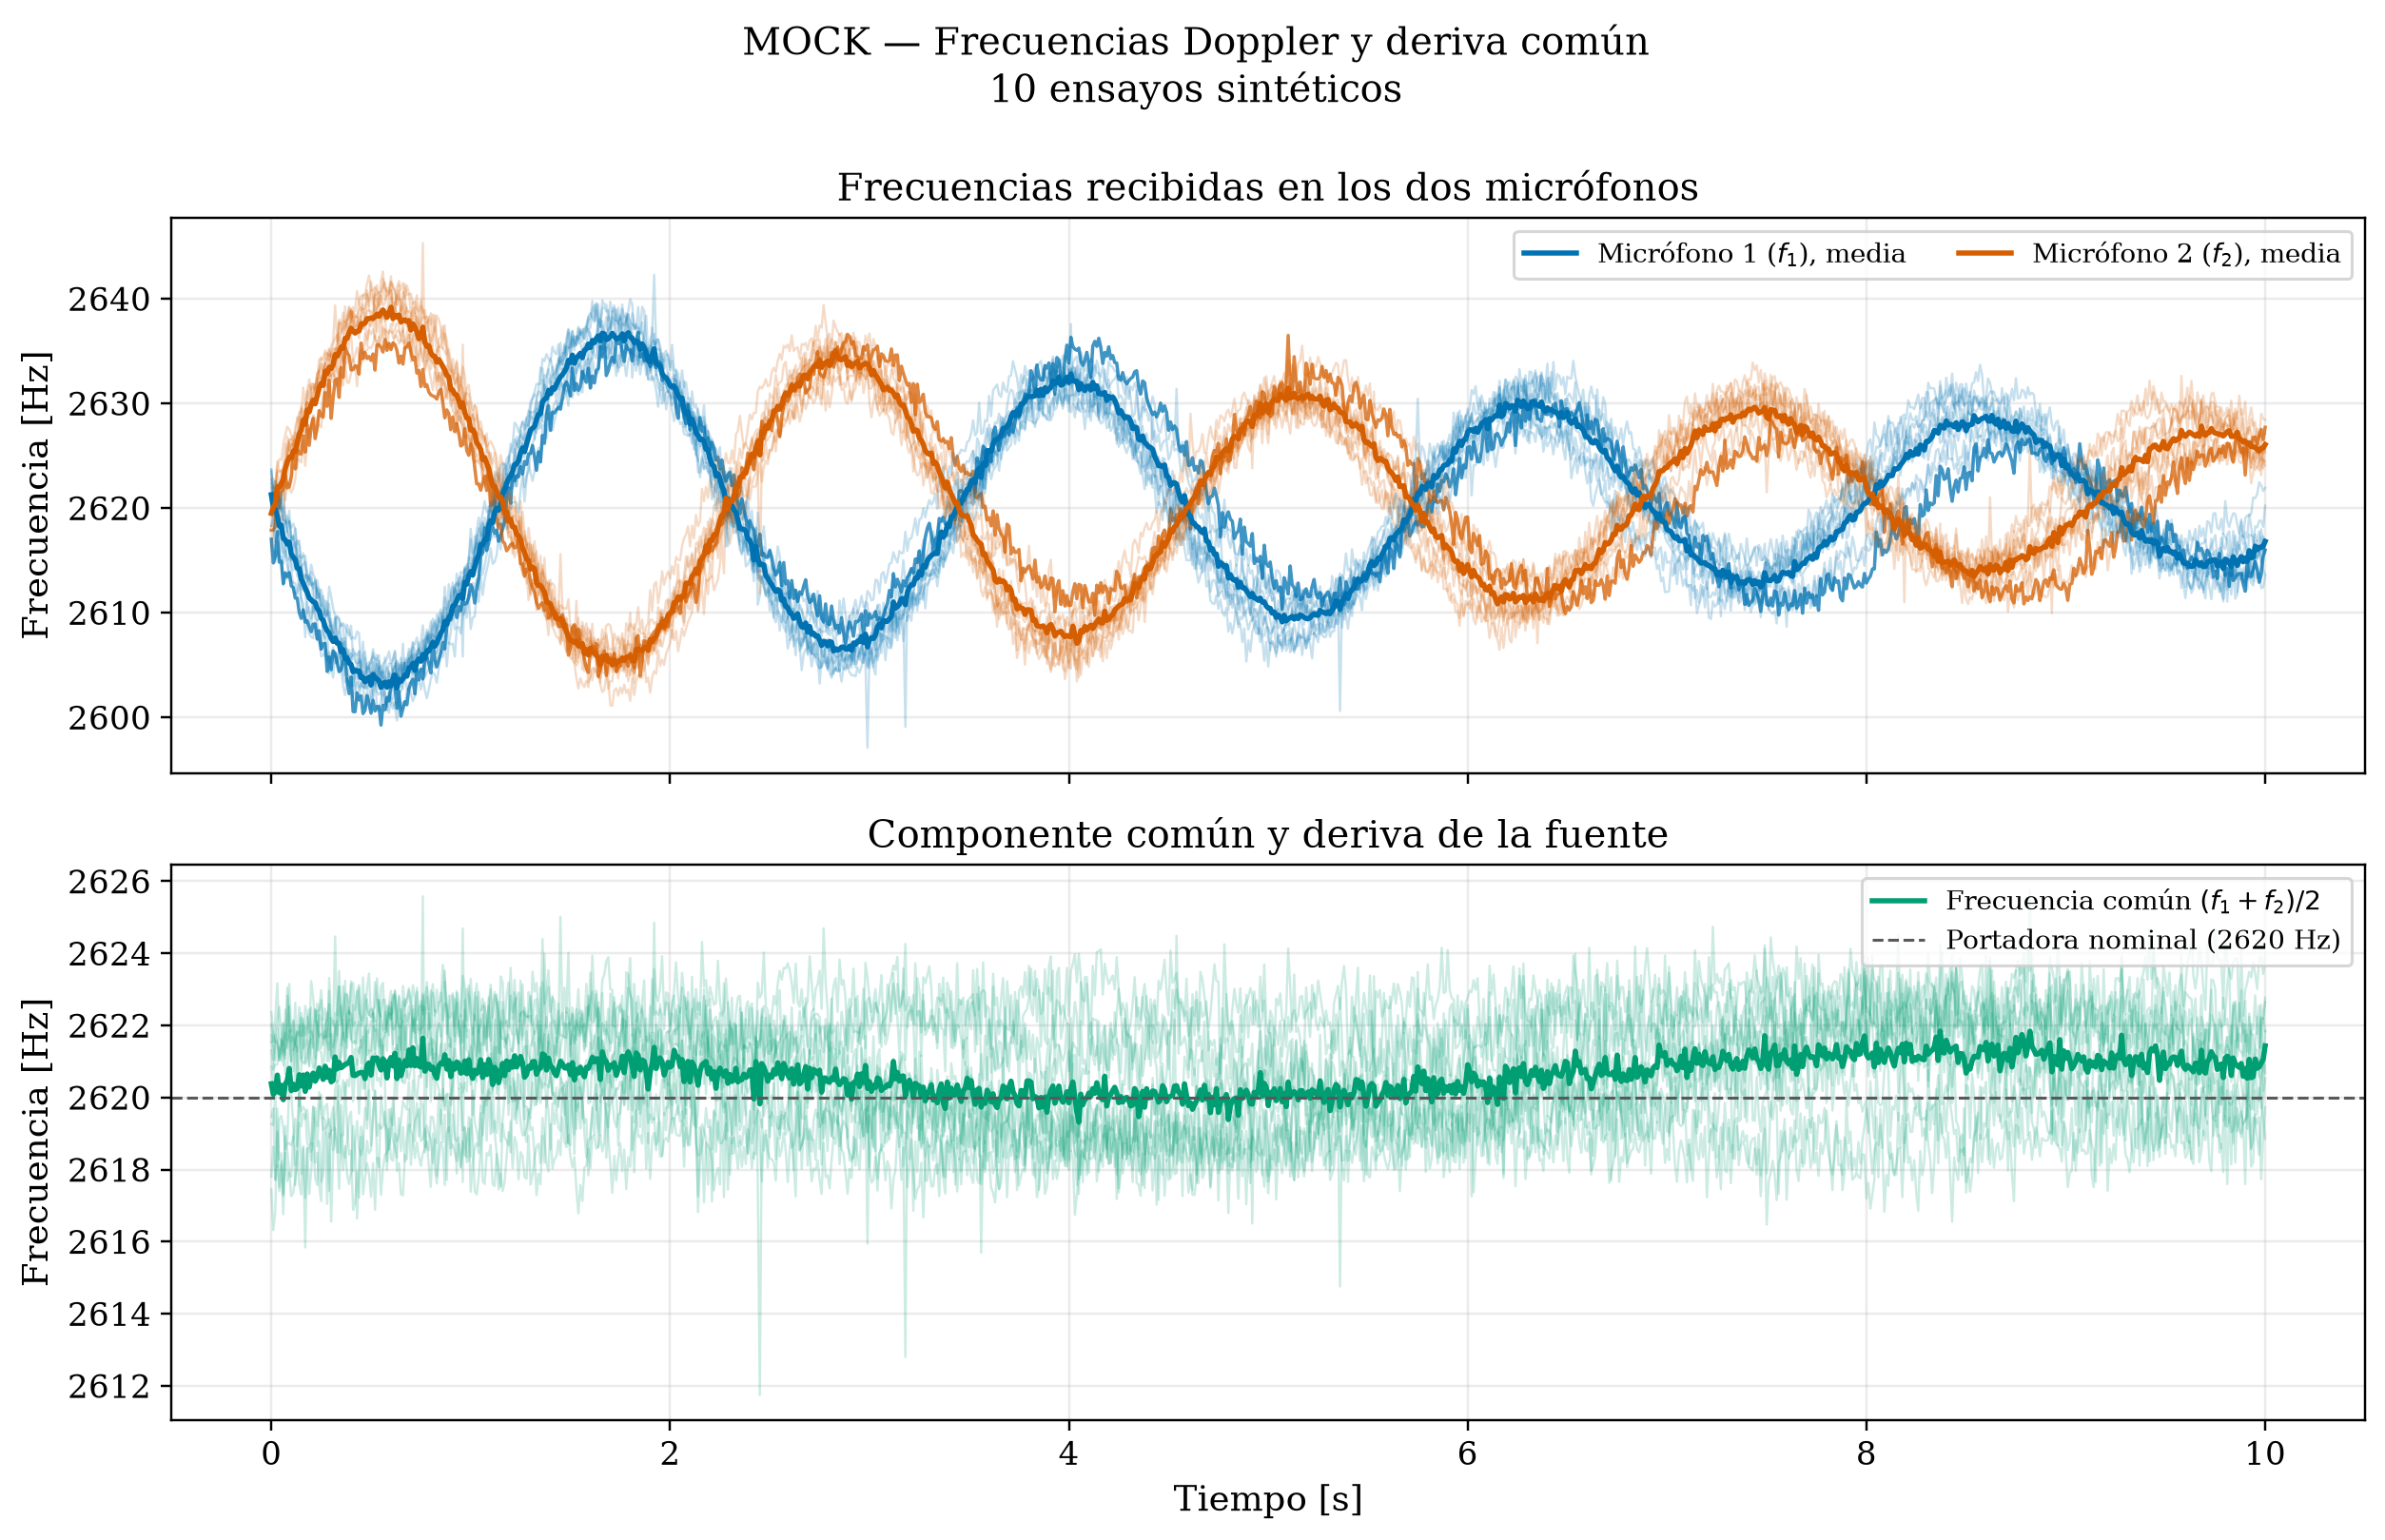
\includegraphics[width=0.98\textwidth]
    {figures/mock_exp03_fig1_doppler_frequencies.png}
    \caption{
        Evolución temporal de las frecuencias Doppler recibidas
        por los dos micrófonos y representación de la componente
        común. Figura MOCK generada con datos sintéticos.
    }
    \label{fig:exp03_frequencies_mock}
\end{figure}

La comparación de las frecuencias recibidas constituye
el punto de partida para separar las contribuciones asociadas
al movimiento de la fuente. En particular, las variaciones
diferenciales entre canales contienen información sobre
la velocidad radial, mientras que las variaciones comunes
pueden reflejar cambios compartidos por ambas observaciones.

La interpretación cuantitativa de estas componentes requiere
aplicar el modelo Doppler desarrollado en el Capítulo 2
y considerar la geometría del montaje. La figura se incluye
para mostrar la presentación prevista del análisis, no
como evidencia de una medición real.

\subsubsection{Reconstrucción y comparación de velocidad}

A partir de las frecuencias estimadas en ambos canales,
el modelo Doppler permite obtener una estimación temporal
de la velocidad de la fuente. Esta magnitud se compara
con la velocidad calculada a partir del seguimiento óptico
realizado mediante Tracker.

La Figura~\ref{fig:exp03_velocity_mock} presenta la estructura
prevista para esta comparación.

\begin{figure}[htbp]
    \centering
    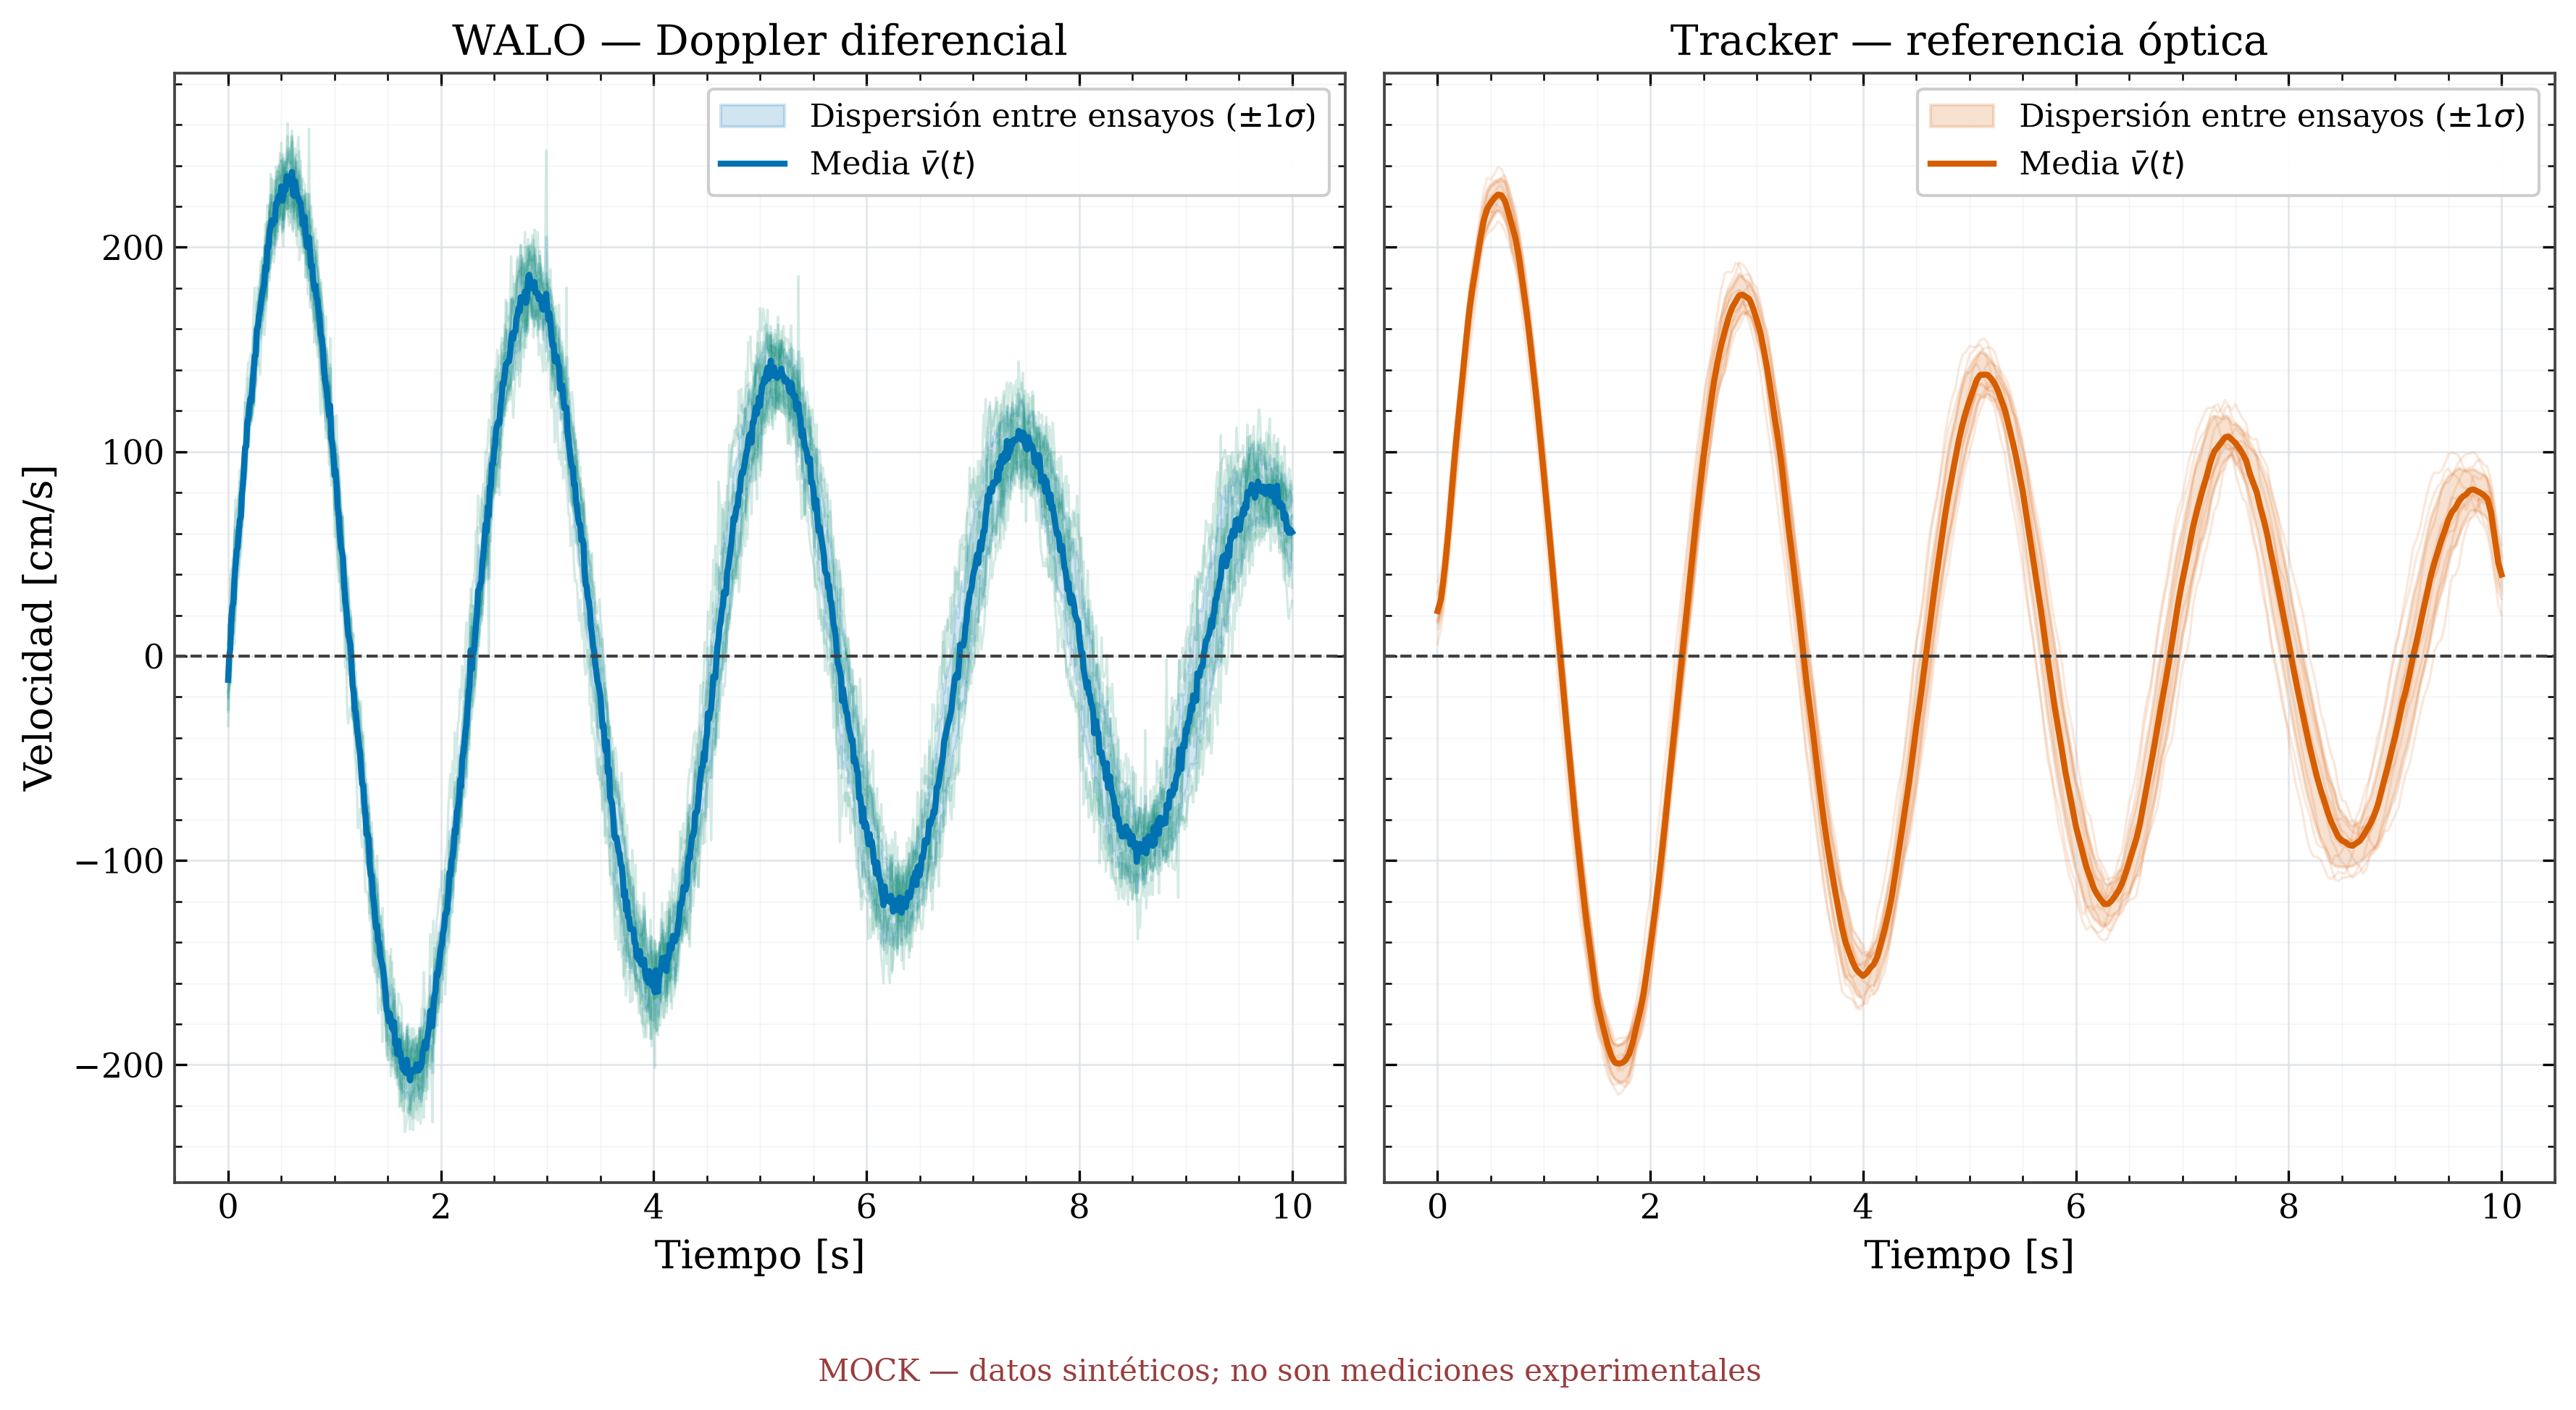
\includegraphics[width=0.98\textwidth]
    {figures/mock_exp03_fig2_velocity_comparison.png}
    \caption{
        Comparación de la velocidad reconstruida mediante
        el modelo Doppler y la velocidad obtenida mediante
        Tracker. Se muestran diez ensayos sintéticos.
        Figura MOCK: los datos no corresponden a mediciones
        experimentales.
    }
    \label{fig:exp03_velocity_mock}
\end{figure}

La comparación entre ambas reconstrucciones permitirá
examinar la correspondencia temporal entre los métodos,
así como las diferencias en amplitud, fase y evolución
de la velocidad durante el movimiento.

La dispersión entre repeticiones también será relevante
para establecer la reproducibilidad del procedimiento.
Una vez disponibles los registros experimentales, esta
comparación podrá complementarse con métricas cuantitativas,
como el error cuadrático medio entre las velocidades
reconstruidas.

En esta etapa, la figura permite visualizar la organización
del resultado que se espera obtener, pero no permite
establecer la precisión real del estimador Doppler.

\subsubsection{Reconstrucción de posición}

La velocidad estimada proporciona una descripción temporal
del movimiento. Para obtener la posición de la fuente
es necesario integrar esta magnitud respecto al tiempo:

\begin{equation}
    x(t) = x(t_0) +
    \int_{t_0}^{t} v(\tau)\,\mathrm{d}\tau.
    \label{eq:exp03_position_integration}
\end{equation}

La reconstrucción depende tanto de la estimación de velocidad
como de la condición inicial empleada para fijar la posición.
Además, cualquier desviación sistemática en la velocidad
puede acumularse durante la integración y producir diferencias
crecientes en la posición reconstruida.

La Figura~\ref{fig:exp03_position_mock} presenta una
visualización sintética de la comparación entre la posición
obtenida mediante WALO y la referencia óptica.

\begin{figure}[htbp]
    \centering
    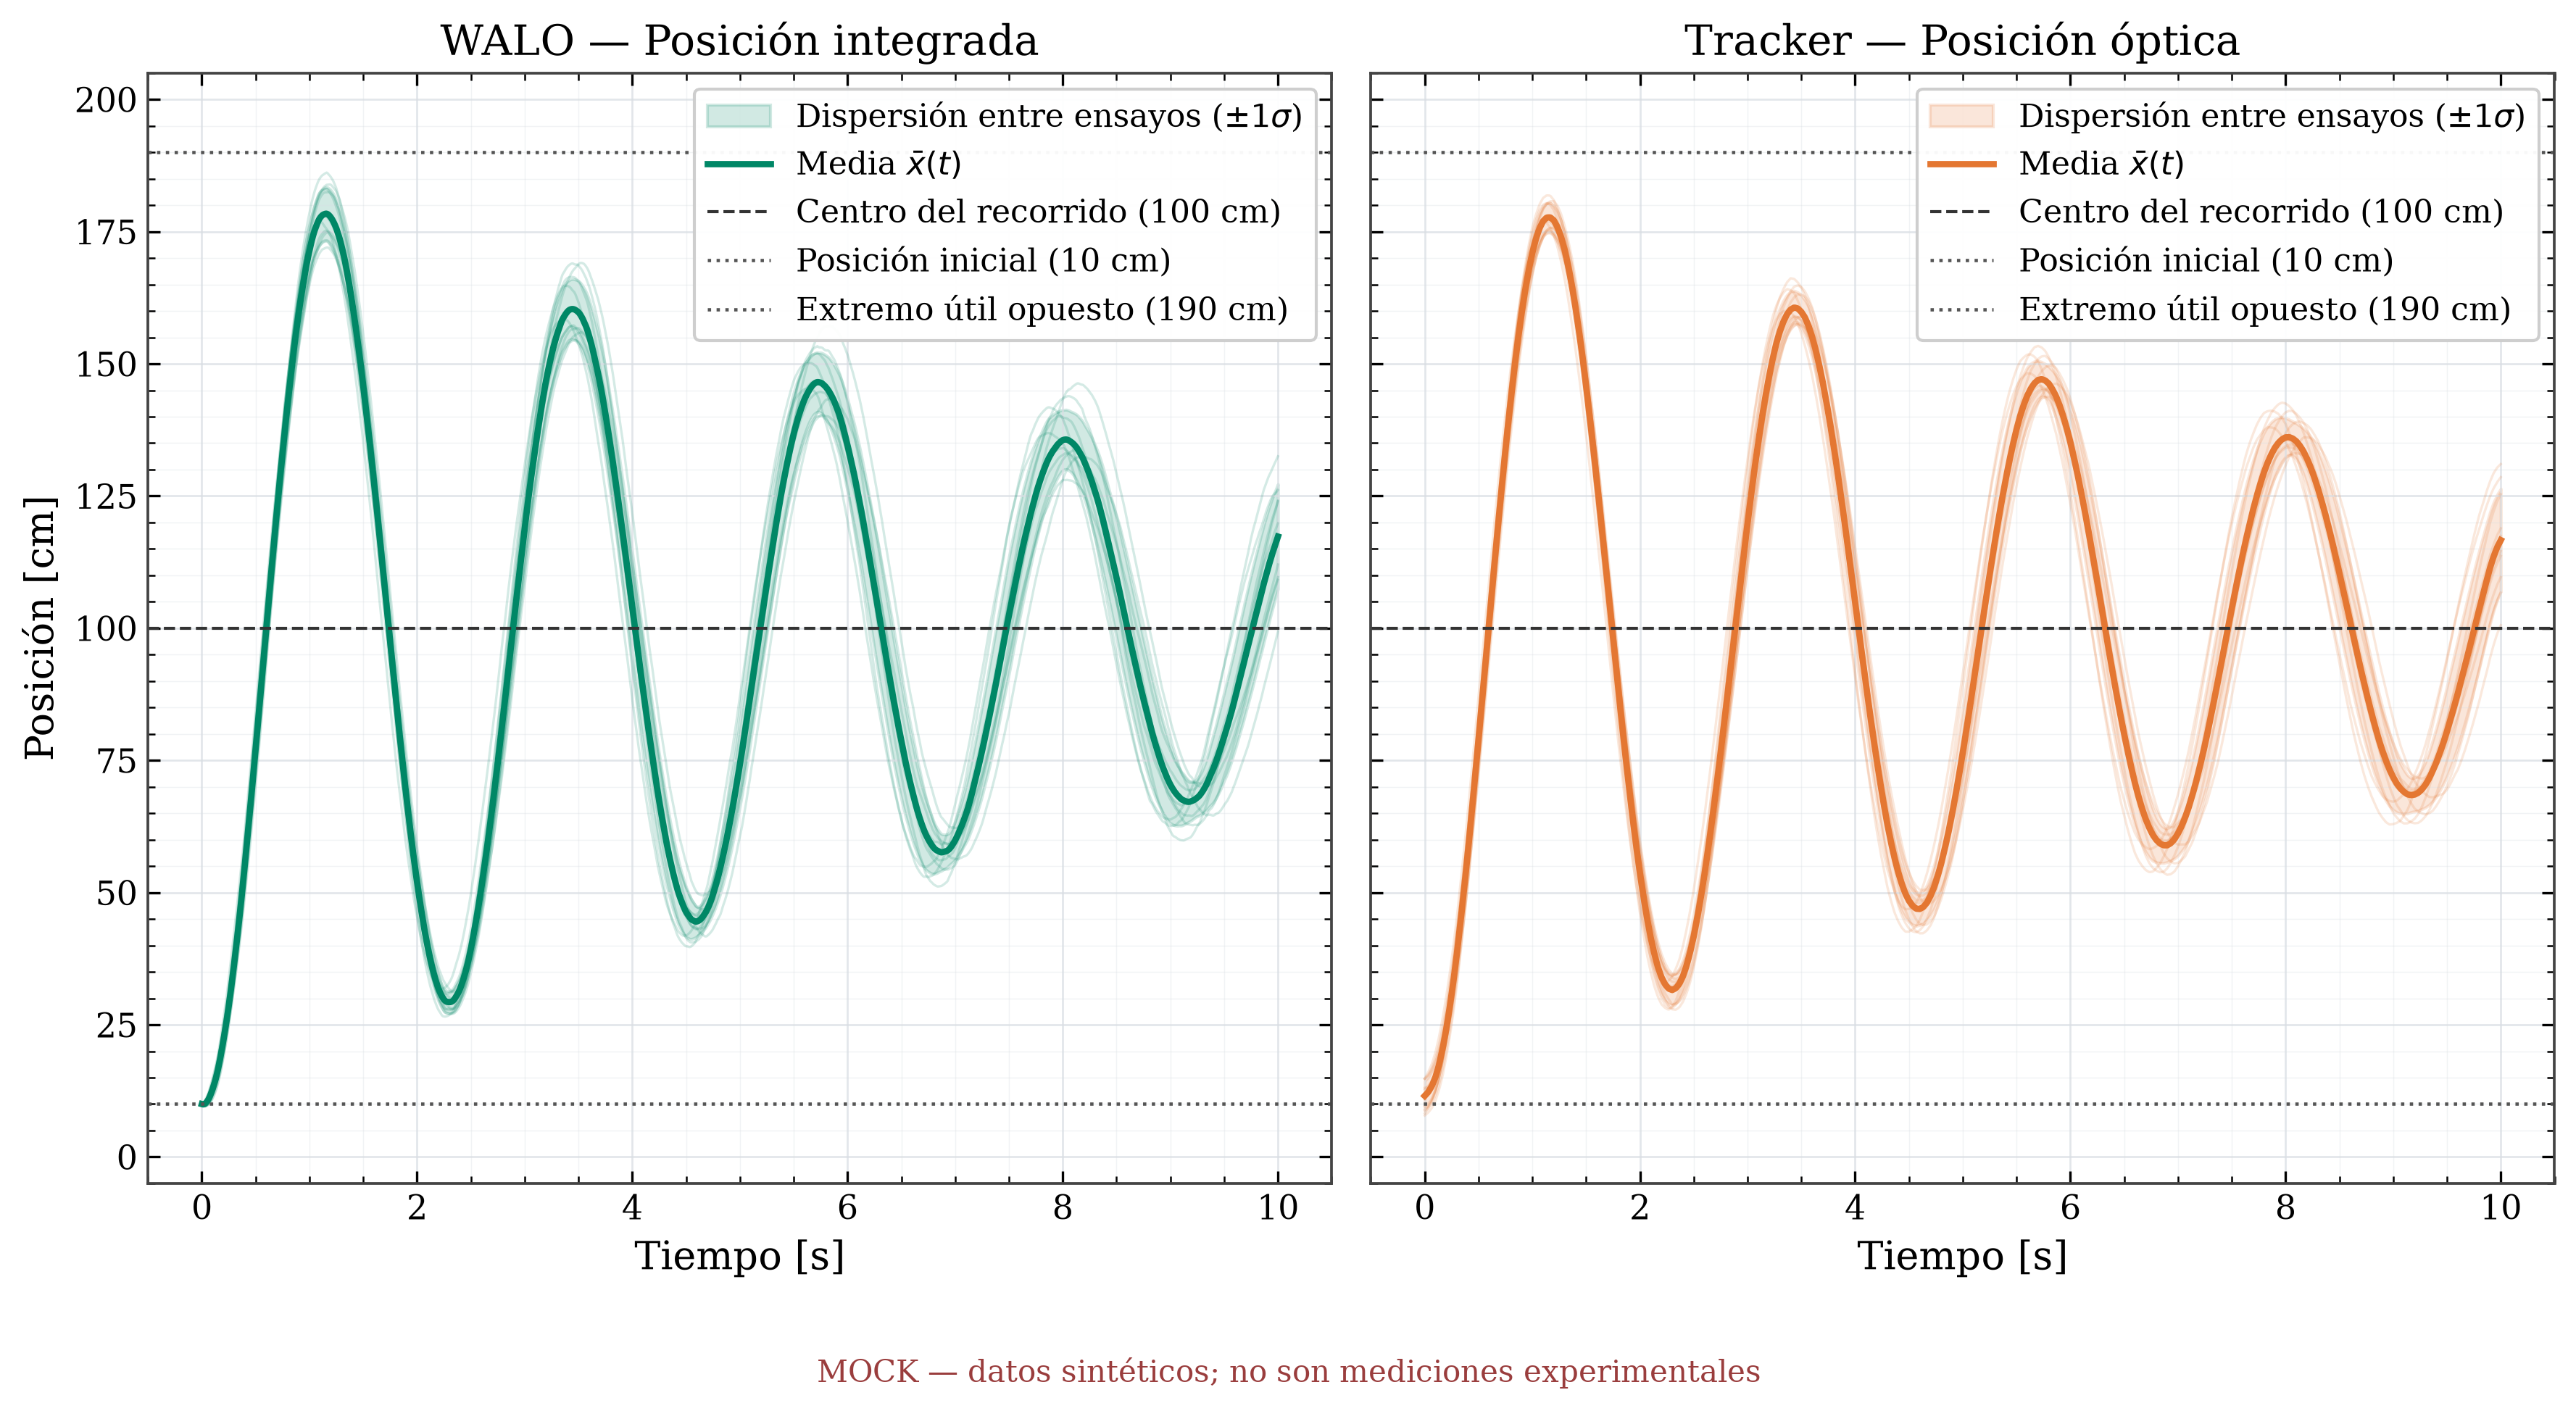
\includegraphics[width=0.98\textwidth]
    {figures/mock_exp03_fig3_position_comparison.png}
    \caption{
        Comparación de la posición reconstruida mediante
        integración de la velocidad Doppler y la posición
        obtenida mediante Tracker. Se muestran diez ensayos
        sintéticos. Figura MOCK: los datos no corresponden
        a mediciones experimentales.
    }
    \label{fig:exp03_position_mock}
\end{figure}

La comparación de posición es especialmente importante
porque permite examinar la propagación de los errores
de velocidad hacia la reconstrucción espacial. Incluso
cuando las diferencias instantáneas de velocidad son
moderadas, su integración puede producir desviaciones
acumulativas o desplazamientos sistemáticos.

Por esta razón, la evaluación de la posición deberá
considerar la condición inicial, el intervalo de integración
y la posible presencia de deriva. La comparación con
Tracker permitirá determinar si la reconstrucción acústica
reproduce adecuadamente la trayectoria observada.

Las figuras de esta sección son visualizaciones sintéticas
destinadas a establecer la presentación del análisis.
No se extraen de ellas métricas de desempeño ni conclusiones
sobre la precisión experimental de WALO.

% ==============================================================================
% 4.5 SÍNTESIS DEL CAPÍTULO
% ==============================================================================

\subsection{Síntesis}
\label{subsec:sintesis_cap4}

Los experimentos presentados abordan de manera complementaria
la obtención de información espacial y cinemática a partir
de señales acústicas. La caracterización radial estudia
la relación entre la respuesta registrada y la distancia;
la evaluación angular compara dos métodos de estimación
de dirección de llegada; y el experimento Doppler extiende
el análisis hacia la reconstrucción temporal del movimiento.

En la evaluación angular, los resultados disponibles muestran
un menor error global para PDoA respecto a TDoA bajo las
condiciones experimentales consideradas. En la caracterización
radial se establece una relación entre la amplitud RMS y
la distancia, junto con una evaluación basada en el tiempo
de llegada.

Finalmente, la reconstrucción cinemática plantea una vía
para obtener velocidad y posición a partir de las frecuencias
recibidas por dos micrófonos. La comparación con Tracker
constituye el procedimiento de validación previsto para
esta etapa.

Las figuras sintéticas incluidas en los apartados de predicción
de distancia y reconstrucción Doppler permiten visualizar
la organización de los resultados que se incorporarán
cuando se disponga de los registros experimentales
correspondientes. Por tanto, la evaluación global del
desempeño de WALO deberá establecerse a partir de esos
datos y de su comparación con las referencias independientes.
